\documentclass[a4paper, utf8]{ctexart}
\usepackage[fontset=Fandol]{ctex}
\usepackage{anyfontsize}
\usepackage{algorithm}
\usepackage{longtable}
\usepackage{abstract}
\usepackage{amsfonts}
\usepackage{appendix}
\usepackage{booktabs}
\usepackage{enumitem}
\usepackage{fancyhdr}
\usepackage{geometry}
\usepackage{graphicx}
\usepackage{tabularx}
\usepackage{listings}
\usepackage{amsmath}
\usepackage{caption}
\usepackage{lipsum}
\usepackage{minted}
\usepackage{xcolor}
\usepackage{array}

\geometry{a4paper,left=31mm,right=31mm,top=25mm,bottom=25mm}
\CTEXsetup[format={\Large \bfseries}]{section}

\setlength{\parindent}{2em}
\pagestyle{fancy}
\fancyhf{}
\fancyhead[L]{并行程序设计与算法实验\ 实验报告}
\fancyhead[R]{Lab6\ Pthreads并行构造}
\fancyhead[C]{}
\fancyfoot[C]{\thepage}
\fancyfoot[L,R]{}

\setCJKfamilyfont{zhsong}[AutoFakeBold = {2.17}]{SimSun}
\renewcommand*{\songti}{\CJKfamily{zhsong}}
\definecolor{LightGray}{gray}{0.9}

\title{\songti \bfseries Lab6\ Pthreads并行构造}
\author{\fangsong 21307210\ \ 傅祉珏}
\date{\fangsong 中山大学计算机学院\ 广东广州\ 510006}

\begin{document}
	
	\begin{titlepage}
		\centering
		\rule{\textwidth}{1pt}
		\vspace{0.02\textheight}
		
		{\LARGE \kaishu 并行程序设计与算法实验\ 实验报告}
		
		\vspace{0.02\textheight}
		
		{\Huge \songti \bfseries Lab6\ Pthreads并行构造}
		
		\vspace{0.025\textheight}
		\rule{0.83\textwidth}{0.4pt}
		\vspace{0.05\textheight} 
		\begin{figure}[htbp]
			\centering
			
\includegraphics[width=8cm, height=8cm]{./figure/计院院徽.jpg}
		\end{figure}
		
		\vspace{0.04\textheight} 
		{\Large 姓名:傅祉珏}
		
		\vspace{0.025\textheight} 
		{\Large 学号:21307210}
		
		\vspace{0.025\textheight} 
		{\Large 专业:计算机科学与技术}
		
		\vspace{0.025\textheight} 
		{\Large Email:futk@mail2.sysu.edu.cn}
		
		\vspace{0.025\textheight} 
		{\Large 完成时间:\today}
		
		\vspace{0.05\textheight} 
		\vfill
		
		{\large \today}
		\vspace{0.1\textheight}
		\rule{\textwidth}{1pt}
	\end{titlepage}
	\let\cleardoublepage\clearpage
	
	\maketitle
	
	\renewcommand{\abstractname}{\large \textbf{摘要}}
	\begin{abstract}
		本实验通过使用Pthreads线程库实现并行化的\verb|for|循环分解、分配与执行机制,探索了并行计算中的任务划分与调度策略。实验的主要目标是实现一个通用的\verb|parallel_for|函数,并通过该函数实现矩阵乘法和热传导模拟问题的并行化求解。通过对比静态调度与动态调度策略,分析了不同线程数和任务规模下的性能表现。实验结果表明,静态调度在大规模任务下能够显著提高计算效率,而动态调度则在小规模任务中表现出更好的灵活性和性能优化。最终,本实验不仅验证了Pthreads并行计算的有效性,也提供了多线程编程中的调度策略选择依据。
		
		\noindent{\textbf{\heiti 关键词:}Pthreads,并行计算,任务调度,静态调度,动态调度。}
	\end{abstract}
	
	\section{实验目的}
	
	本实验旨在掌握基于Pthreads线程库的并行程序设计方法,重点实现仿照OpenMP的\verb|omp_parallel_for|机制的并行\verb|for|循环分解、分配与执行功能。通过设计并实现一个通用的\verb|parallel_for|函数,支持根据循环起始索引、终止索引、自增步长、线程数及具体执行内容等参数,自动进行任务划分与多线程并行调度,培养并行计算中面向通用接口设计与模块化实现的能力。实验要求将\verb|parallel_for|函数封装为动态链接库(\verb|.so|文件),实现通用调用。
	
	在应用层面,实验通过将传统串行矩阵乘法程序改造为基于\verb|parallel_for|接口的并行矩阵乘法,检验并行构造的正确性与性能表现。同时,进一步要求以加热板(heated plate)热传导模拟问题为案例,改造原有的基于OpenMP的并行实现,使其基于Pthreads与\verb|parallel_for|机制进行并行计算,分析不同线程数和任务划分策略下的性能变化。通过本实验,能够系统理解并行循环执行机制的基本原理,掌握Pthreads多线程编程方法,提升针对实际数值计算任务设计高效并行解决方案的能力。
	
	\section{实验过程}
	
	\subsection{基于Pthreads的并行\texttt{for}循环分解、分配、执行机制构造}
	
	在本实验中,首先构建了一个基于Pthreads的并行for循环分解、分配与执行机制。核心目标是实现一个能够支持多线程并行化for循环的\verb|parallel_for|函数,该函数能够通过指定的调度策略来动态或静态地分配任务,确保任务能够在多个线程之间高效分配与执行。
	
	实验的第一步是设计和实现\verb|parallel_for|函数的结构。为了支持多线程并行执行,每个线程的执行任务由一个结构体\verb|ThreadArgs|进行传递,该结构体包含了线程ID、任务的起始与结束索引、任务增量、执行的函数指针等信息。通过这种方式,能够确保每个线程都能够根据自身的参数执行特定的任务,而不会发生冲突。
	
	\begin{minted}[baselinestretch=1, framesep=0mm, escapeinside=||]{cpp}
typedef struct {
    int thread_id;
    int start;
    int end;
    int inc;
    void *(*functor)(int, void*);
    void *arg;
    schedule_t schedule;
    int *shared_idx;
    pthread_mutex_t *lock;
} ThreadArgs;
	\end{minted}
	
	在实现任务分配与执行机制时,考虑到任务的负载均衡与线程同步,设计了两种主要的调度策略:静态调度与动态调度。静态调度通过均匀分配任务的迭代次数给各个线程,确保每个线程处理的任务数量大致相同,从而实现负载均衡。在静态调度中,每个线程根据分配的任务范围执行循环,确保各个线程并行执行不同部分的任务。
	
	与静态调度不同,动态调度采用了任务队列的方式,每个线程从共享的任务队列中动态获取任务并执行。这种方式适用于任务量较大且任务执行时间不均衡的场景。为了避免多个线程同时访问共享任务队列时发生数据竞争,采用了互斥锁机制对共享变量进行保护,确保每次只有一个线程能够更新任务队列的索引。
	
	\begin{minted}[baselinestretch=1, framesep=0mm, escapeinside=||]{cpp}
void *thread_func_static(void *arg) {
    ThreadArgs *args = (ThreadArgs *)arg;
    for (int i = args->start; i < args->end; i += args->inc) {
        args->functor(i, args->arg);
    }
    return NULL;
}

void *thread_func_dynamic(void *arg) {
    ThreadArgs *args = (ThreadArgs *)arg;
    while (1) {
        int idx;
        pthread_mutex_lock(args->lock);
        idx = *(args->shared_idx);
        *(args->shared_idx) += args->inc;
        pthread_mutex_unlock(args->lock);

        if (idx >= args->end) break;
        args->functor(idx, args->arg);
    }
    return NULL;
}
	\end{minted}
	
	在完成任务分配和线程创建之后,程序通过\verb|pthread_join|确保所有线程执行完毕。\verb|pthr|\ \verb|ead_join|函数能够阻塞主线程,直到所有子线程完成工作。这样做能够确保主线程在所有并行任务完成后继续进行后续操作。
	
	最终,实验中通过调用并行化的\verb|parallel_for|函数来测试不同数量线程在静态与动态调度下的性能表现。通过这些实验,验证了并行化执行的正确性和效率,确保了多线程任务能够正确地分配与执行,同时提升了任务处理的并行效率。
	
	\subsection{\texttt{parallel\_for}并行应用}
	
	在本实验中,应用\verb|parallel_for|函数对热板问题(heated plate problem)进行了并行化求解。热板问题的目标是求解一个二维矩阵上的热传导问题,其中矩阵的边界条件已知,初始条件设定为矩阵内部的所有值为常数。通过迭代计算矩阵内每个点的温度值,直到满足预定的精度要求。
	
	实验的第一步是设置热板的边界条件。通过调用\verb|parallel_for|函数,分别为热板的上下边界和左右边界设置固定的温度值。在这一步骤中,\verb|parallel_for|通过静态或动态调度的方式,将边界的设置任务分配给多个线程进行并行执行。每个线程根据分配的任务范围更新相应的边界温度。
	
	\begin{minted}[baselinestretch=1, framesep=0mm, escapeinside=||]{cpp}
void set_boundary_left_right(int i, void* arg) {
    double (*w)[N] = (double (*)[N])arg;
    w[i][0] = 100.0;
    w[i][N-1] = 100.0;
}

void set_boundary_top_bottom(int j, void* arg) {
    double (*w)[N] = (double (*)[N])arg;
    w[M-1][j] = 100.0;
    w[0][j] = 0.0;
}

typedef struct {
    double (*w)[N];
    double* boundary_sum;
} BoundarySumArg;

void sum_boundary_left_right(int i, void* arg) {
    BoundarySumArg* bsa = (BoundarySumArg*)arg;
    *(bsa->boundary_sum) += bsa->w[i][0] + bsa->w[i][N-1];
}

void sum_boundary_top_bottom(int j, void* arg) {
    BoundarySumArg* bsa = (BoundarySumArg*)arg;
    *(bsa->boundary_sum) += bsa->w[M-1][j] + bsa->w[0][j];
}
	\end{minted}
	
	接下来,实验进入计算热板内点的初始值阶段。为了满足热传导的初始条件,矩阵内部的每个点的温度设置为平均值。这个步骤同样使用了\verb|parallel_for|来进行并行化操作。每个线程处理不同的矩阵行,更新矩阵内的点的温度值。
	
	\begin{minted}[baselinestretch=1, framesep=0mm, escapeinside=||]{cpp}
typedef struct {
    double (*w)[N];
    double mean;
} InitInnerArg;

void initialize_inner(int i, void* arg) {
    InitInnerArg* iia = (InitInnerArg*)arg;
    for (int j = 1; j < N-1; j++) {
        iia->w[i][j] = iia->mean;
    }
}
	\end{minted}
	
	然后,进入核心的计算迭代阶段。在每次迭代中,首先需要将当前温度矩阵$w$的值复制到$u$矩阵中,以便进行新的计算。接着,按照热传导公式更新矩阵内点的温度值,公式为每个点的温度值是其上下左右四个相邻点温度值的平均值。这一计算也通过\verb|parallel_for|函数实现,分配给多个线程并行执行。
	
	\begin{minted}[baselinestretch=1, framesep=0mm, escapeinside=||]{cpp}
typedef struct {
    double (*w)[N];
    double (*u)[N];
} CopyArg;

void copy_matrix(int i, void* arg) {
    CopyArg* ca = (CopyArg*)arg;
    for (int j = 0; j < N; j++) {
        ca->u[i][j] = ca->w[i][j];
    }
}

void compute_new_values(int i, void* arg) {
    CopyArg* ca = (CopyArg*)arg;
    for (int j = 1; j < N-1; j++) {
        ca->w[i][j] = 0.25 * (ca->u[i-1][j] + ca->u[i+1][j]
                            + ca->u[i][j-1] + ca->u[i][j+1]);
    }
}
	\end{minted}
	
	每次迭代后,需要计算当前迭代与前一迭代之间的最大温度差异,以判断是否已经满足精度要求。当最大温差小于预设的阈值时,认为热传导过程已经收敛,计算终止。为了高效地计算最大差异值,\verb|parallel_for|被用于并行计算每个点的差异,并找出所有点中的最大差异。
	
	整个计算过程持续迭代,直到满足精度要求。在每次迭代完成后,程序都会更新最大差异值,并继续进行下一次迭代,直到达到预设的精度阈值。
	
	\begin{minted}[baselinestretch=1, framesep=0mm, escapeinside=||]{cpp}
typedef struct {
    double (*w)[N];
    double (*u)[N];
    double* max_diff;
} DiffArg;

void compute_max_diff(int i, void* arg) {
    DiffArg* da = (DiffArg*)arg;
    double local_diff = 0.0;
    for (int j = 1; j < N-1; j++) {
        double temp = fabs(da->w[i][j] - da->u[i][j]);
        if (temp > local_diff) {
            local_diff = temp;
        }
    }
    if (local_diff > *(da->max_diff)) {
        *(da->max_diff) = local_diff;
    }
}
	\end{minted}
	
	最终,实验通过记录每次实验的计算时间和迭代次数,评估并行计算的性能表现。通过调整线程数和调度策略,观察并行计算在不同配置下的时间消耗与效率,并进行性能对比分析。实验结果表明,随着线程数的增加,尤其是在较大矩阵和较高线程数下,动态调度能够更好地平衡负载,提高计算效率,减少计算时间。
	
	\section{实验结果}
	
	\subsection{基于Pthreads的并行\texttt{for}循环分解、分配、执行机制构造}
	
	在本实验中,我们使用Pthreads并行框架对一个大型计算任务进行了分解、分配和执行,主要通过并行化for循环来提升计算效率。实验结果展示了不同任务规模和线程数的性能表现。通过对比静态调度和动态调度策略下的执行时间,我们可以清晰地看到并行化带来的加速效益,以及不同调度策略和线程数的影响。
	
	\begin{figure}[htbp]
		\centering
		\begin{minipage}{.45\textwidth}
			\centering
			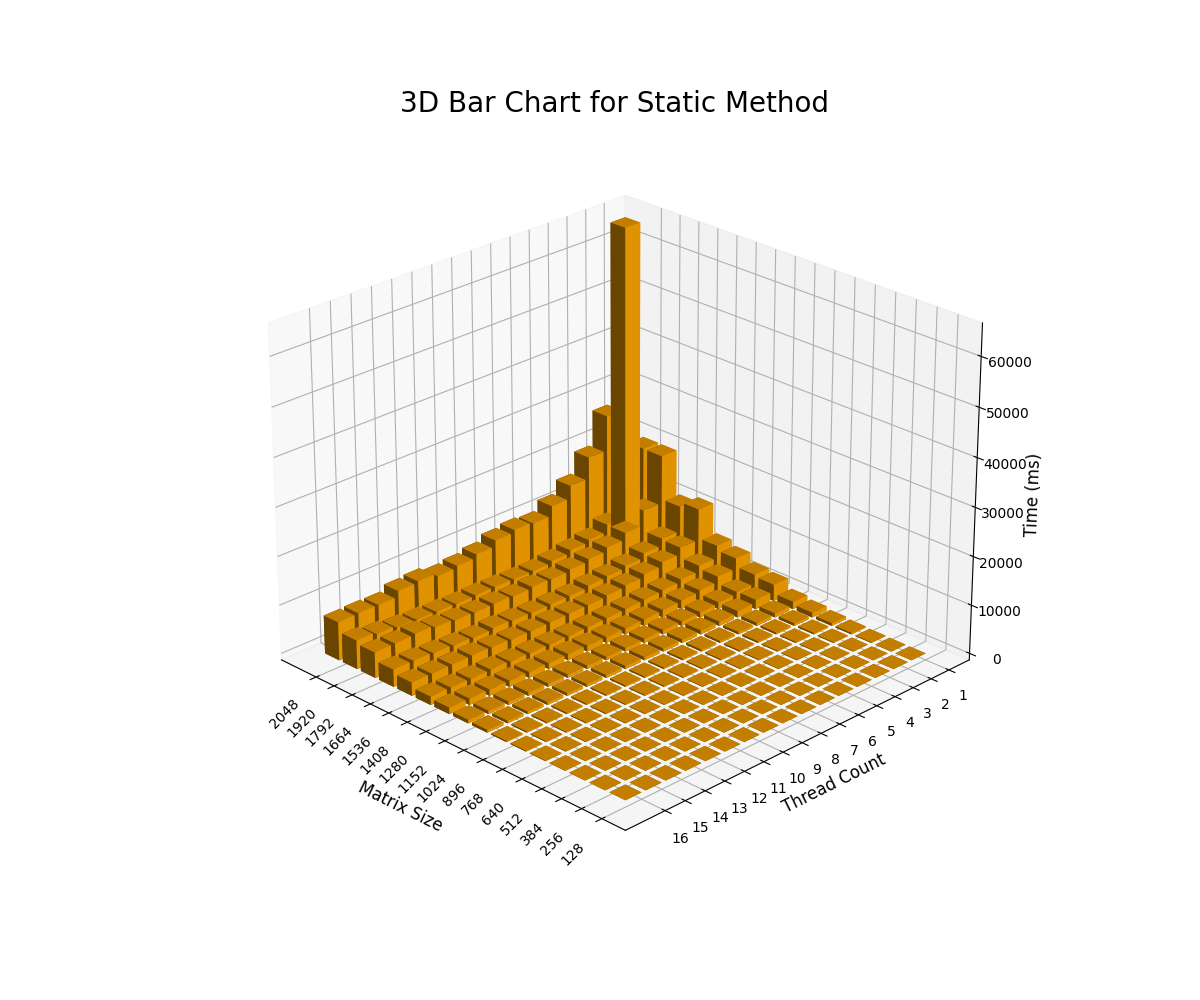
\includegraphics[width=.8\textwidth]{./figure/static_barchart.png}
			\caption{静态调度性能柱状图}
		\end{minipage}
		\begin{minipage}{.45\textwidth}
			\centering
			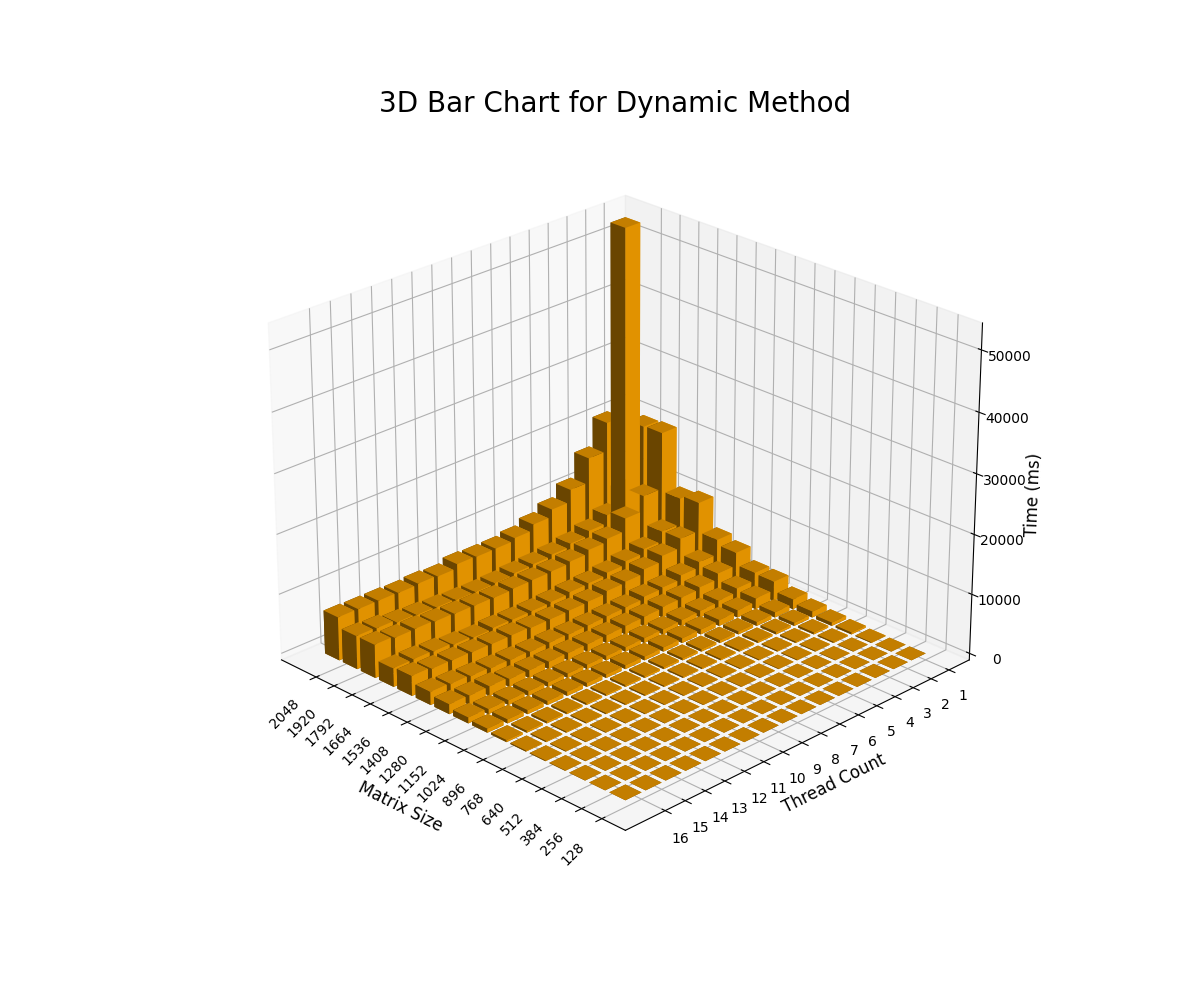
\includegraphics[width=.8\textwidth]{./figure/dynamic_barchart.png}
			\caption{动态调度性能柱状图}
		\end{minipage}
	\end{figure}
	
	首先,在静态调度(\verb|STATIC|)策略下,我们观察到随着线程数的增加,执行时间逐步降低。例如,对于输入大小为$128$的任务,单线程执行时间为$4.79$毫秒,而随着线程数从$1$增加到$16$,执行时间下降至$1.01$毫秒。对于更大规模的任务(如$2048$的输入大小),执行时间从$65157.8$毫秒(单线程)下降到$7882.31$毫秒(16线程)。这一趋势表明,增加线程数可以显著提升计算效率,尤其是在大任务规模下,执行时间的减少更加明显。
	
	然而,并非所有情况下增加线程数都会带来线性加速。在一些任务规模较小的情况下(如$128$),线程数增加后,执行时间有时会略有波动。例如,$128$大小的任务在$16$线程时的执行时间为$1.01$毫秒,而$15$线程时的时间为$1.18$毫秒,这表明在某些情况下,线程数的增加可能会导致系统资源的调度开销增大,从而影响性能。
	
	对于动态调度(\verb|DYNAMIC|)策略,执行时间普遍低于静态调度。在$128$大小的任务中,\verb|DYNAMIC|策略的执行时间随着线程数的增加而逐步降低,最终在$8$线程时,执行时间达到最小值$0.95$毫秒,比静态调度的最优结果($1.01$毫秒)更快。整体来看,动态调度能够根据任务的计算需求和资源分配情况更加灵活地调整线程分配,进一步优化性能。
	
	\begin{figure}[htbp]
		\centering
		\begin{minipage}{.45\textwidth}
			\centering
			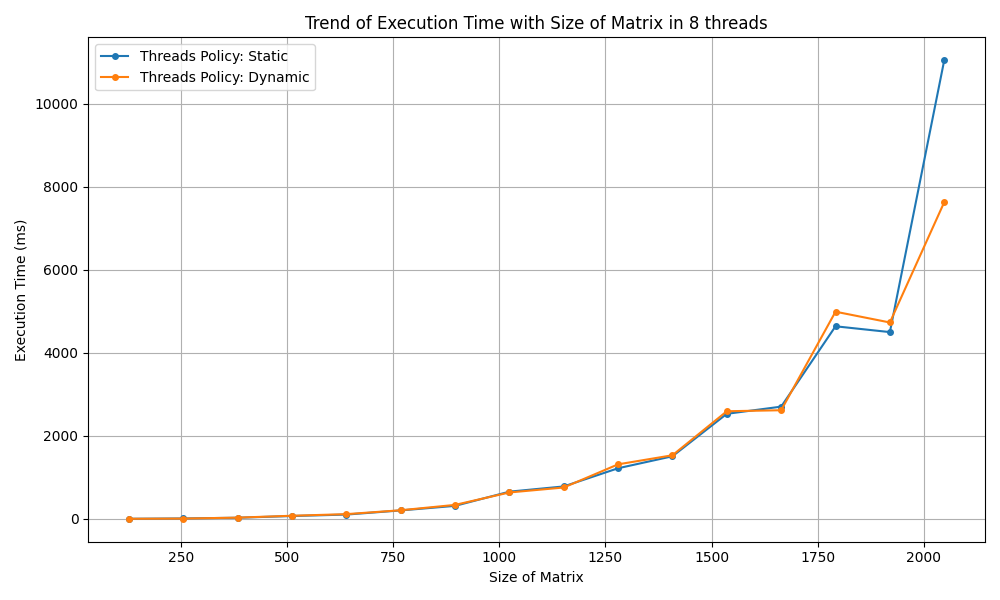
\includegraphics[width=.8\textwidth]{./figure/method_time_trend.png}
			\caption{调度方式性能对比图}
		\end{minipage}
		\begin{minipage}{.45\textwidth}
			\centering
			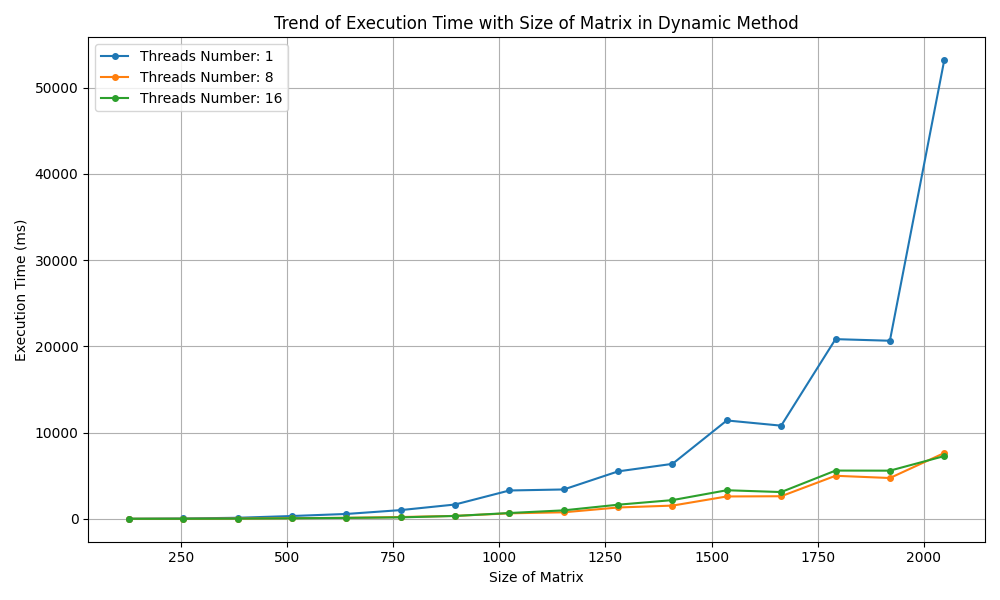
\includegraphics[width=.8\textwidth]{./figure/threads_time_trend.png}
			\caption{线程数性能对比图}
		\end{minipage}
	\end{figure}
	
	总的来说,通过Pthreads并行化\verb|for|循环并结合不同的调度策略,我们能够有效地提升计算效率。对于大规模任务,采用更多的线程和静态调度策略可以显著减少执行时间;而对于小规模任务,动态调度策略能够更好地适应不同的负载情况,进一步提升性能。在实际应用中,选择合适的线程数和调度策略对于优化并行计算的性能至关重要。
	
	\subsection{\texttt{parallel\_for}并行应用}
	
	在本实验中,我们使用了Pthreads的\verb|parallel_for|和OpenMP两种并行化技术对$500\times500$大小的矩阵进行并行计算,并观察了不同线程数和调度策略下的性能表现。
	
	\begin{figure}[htbp]
		\centering
		\begin{minipage}{.45\textwidth}
			\centering
			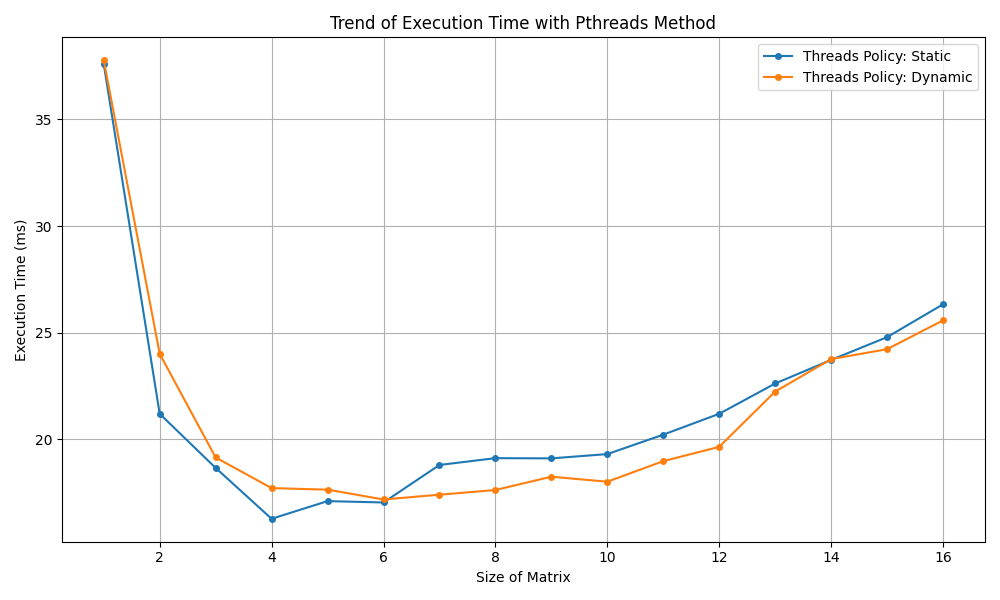
\includegraphics[width=.8\textwidth]{./figure/pthreads_time_trend.png}
			\caption{Pthreads性能趋势图}
		\end{minipage}
		\begin{minipage}{.45\textwidth}
			\centering
			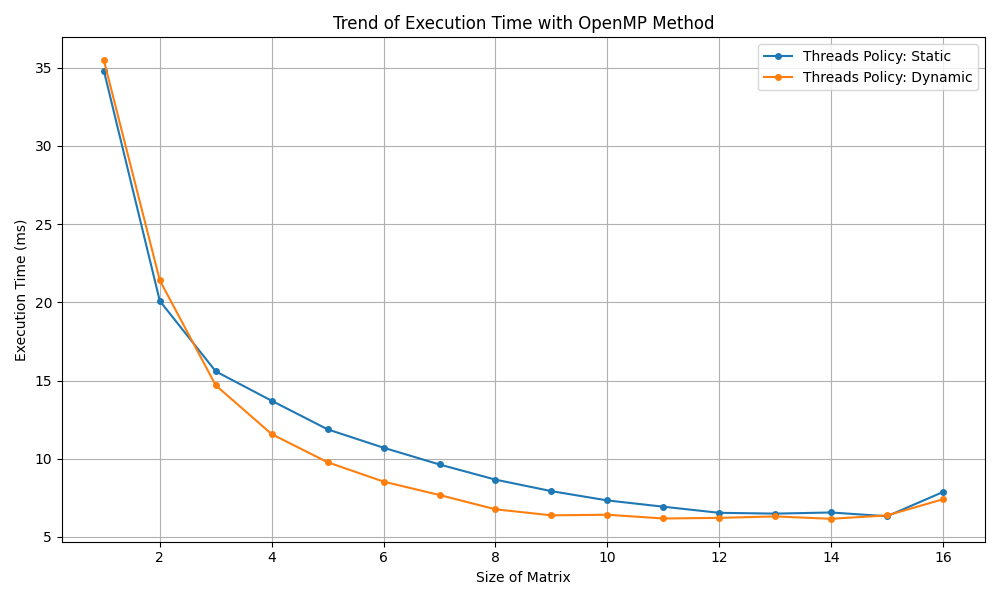
\includegraphics[width=.8\textwidth]{./figure/openmp_time_trend.png}
			\caption{OpenMP性能趋势图}
		\end{minipage}
	\end{figure}
	
	在Pthreads的\verb|parallel_for|应用中,随着线程数的增加,计算时间呈现一定程度的下降。当线程数为$1$时,静态调度的计算时间为$37.60$秒,动态调度的计算时间为$37.78$秒,而当线程数增加到$2$时,静态调度的计算时间降至$21.20$秒,动态调度的计算时间为$24.01$秒。这种趋势在不同线程数下持续存在,尤其是当线程数增加到$6$或更高时,静态调度的计算时间逐渐趋于稳定,维持在约$17$秒左右,动态调度的计算时间则在$17$秒到$18$秒之间波动。然而,超过$12$个线程时,性能提升不再明显,反而有所回升,这表明过多线程可能导致线程调度的开销增加,进而影响性能的提升。
	
	相比之下,使用OpenMP时,性能提升更加显著。对于$1$个线程的情况,静态调度的计算时间为$34.81$秒,动态调度的计算时间为$35.47$秒;当线程数增至$2$时,静态调度的时间降至$20.08$秒,动态调度为$21.40$秒。随着线程数的增加,OpenMP的计算时间进一步缩短,$8$个线程时,静态调度的时间为$8.66$秒,动态调度为$6.77$秒,$16$个线程时,静态调度的计算时间为$7.87$秒,动态调度为$7.41$秒,表现出明显的加速效果。
	
	\begin{figure}[htbp]
		\centering
		\begin{minipage}{.45\textwidth}
			\centering
			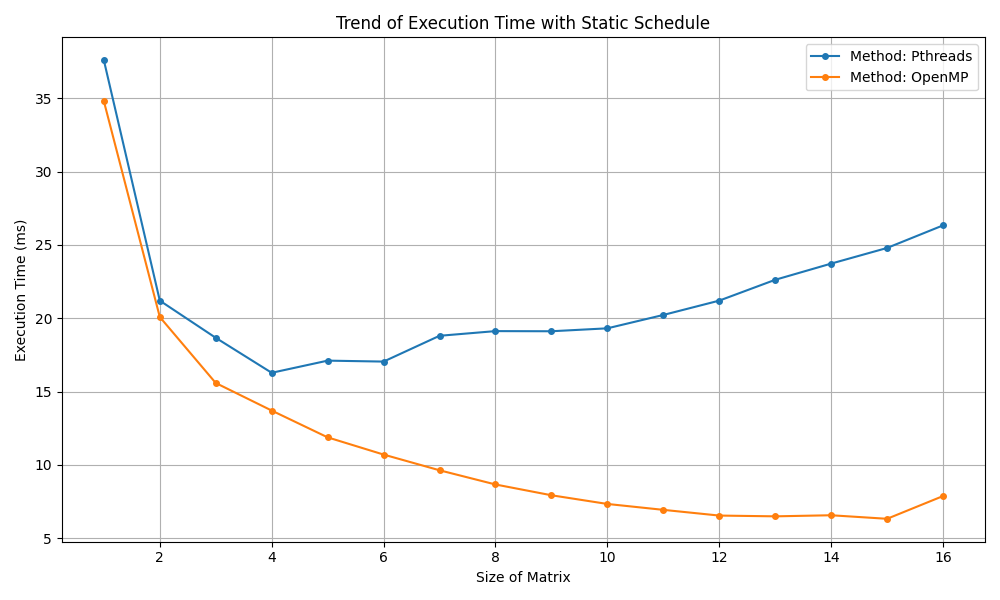
\includegraphics[width=.8\textwidth]{./figure/static_time_trend.png}
			\caption{静态调度性能对比图}
		\end{minipage}
		\begin{minipage}{.45\textwidth}
			\centering
			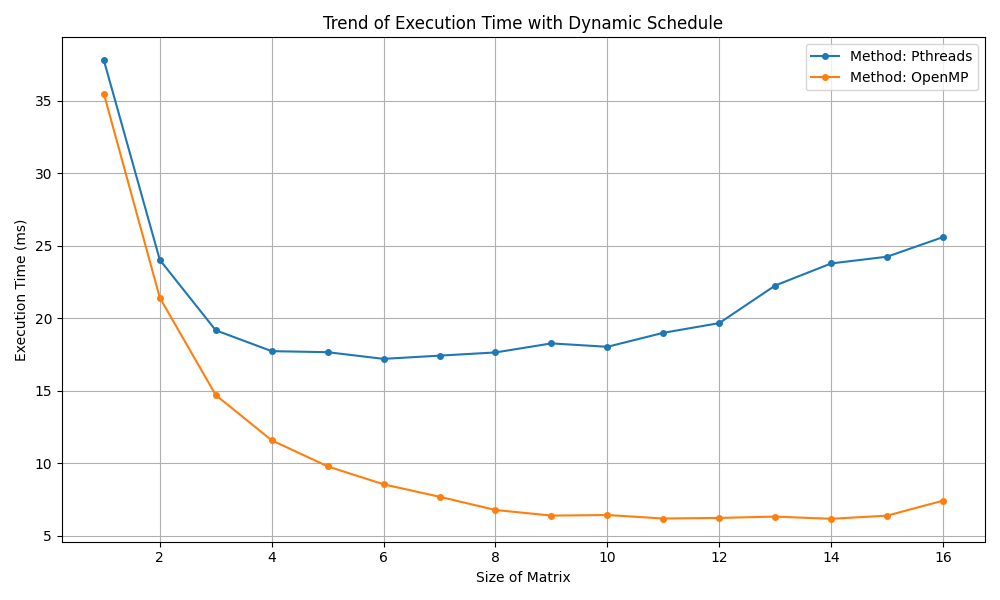
\includegraphics[width=.8\textwidth]{./figure/dynamic_time_trend.png}
			\caption{动态调度性能对比图}
		\end{minipage}
	\end{figure}
	
	综合来看,OpenMP在本实验中相较于Pthreads表现出更优的性能,尤其在较高线程数下,其加速效果更加明显,而Pthreads的性能提升在$16$个线程后趋于平缓。此外,动态调度并未显著提升性能,静态调度在大多数情况下表现更为稳定。因此,选择合适的线程数和调度策略对实现最佳性能至关重要。
	
	\subsection{\texttt{parallel\_for}性能分析}
	
	通过对不同矩阵规模和线程数量下程序执行时间的测量与分析,可以看出程序的性能表现与问题规模和线程配置密切相关。整体而言,随着矩阵规模的增大,程序执行时间呈显著上升趋势,这与计算量的增长直接相关。例如,矩阵规模从2增长到512时,单线程下的运行时间从约0.4秒增加至超过240秒,体现了矩阵计算复杂度的指数级增长。
	
	\begin{figure}[htbp]
		\centering
		\begin{minipage}{.27\textwidth}
			\centering
			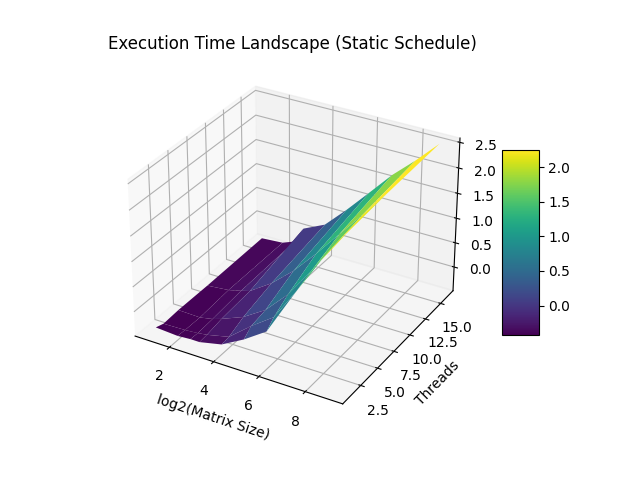
\includegraphics[width=\textwidth]{./figure/TimeLandscape.png}
			\caption{时间曲面图}
		\end{minipage}
		\begin{minipage}{.35\textwidth}
			\centering
			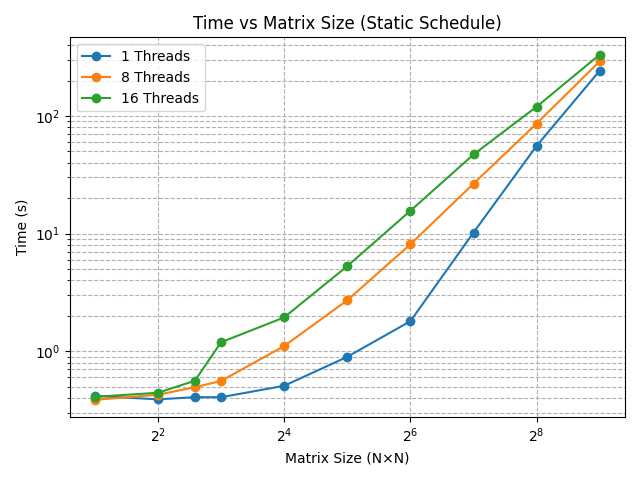
\includegraphics[width=.8\textwidth]{./figure/TimevsSize.png}
			\caption{时间随规模增长趋势图}
		\end{minipage}
		\begin{minipage}{.35\textwidth}
			\centering
			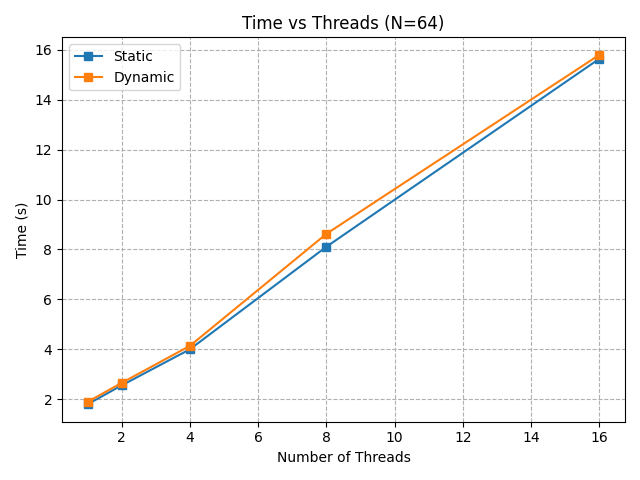
\includegraphics[width=.8\textwidth]{./figure/TimevsThreads.png}
			\caption{时间随线程增长趋势图}
		\end{minipage}
	\end{figure}
	
	在多线程性能方面,结果显示线程数增加并未显著降低程序的执行时间,甚至在某些情况下出现性能退化的现象。对于小规模矩阵(如2),增加线程数对加速效果不明显,执行时间变化较小,这可能是由于线程创建和管理的开销相对于计算量较大,导致并行效率不高。随着矩阵规模增大,线程数量对性能的影响变得更加复杂。在中等规模(如128)时,增加线程数在一定程度上延长了执行时间,表明线程间同步和资源争用可能成为性能瓶颈。尤其是在高线程数(如16线程)配置下,执行时间明显高于低线程数,体现出并行化过程中存在的负载不均衡和调度开销问题。
	
	此外,调度策略(静态调度与动态调度)对程序性能的影响也较为有限,且在多数测试场景中表现出类似的执行时间,说明调度策略并非影响本实验中程序性能的关键因素。值得注意的是,在大规模矩阵和高线程数条件下,动态调度偶尔带来轻微性能波动,但总体趋势与静态调度相近。
	
	综上所述,本次实验的性能分析揭示了该Pthreads并行构造方案在实际运行中的瓶颈和不足。当前的并行实现对于小规模问题存在线程开销掣肘,而在大规模任务中,多线程带来的资源竞争和调度复杂性限制了加速效果,甚至导致性能下降。这提示未来优化方向应着重于提升线程负载均衡、减少同步开销及优化任务划分策略,以发挥多核处理器的真正性能潜力。
	
	\subsection{\texttt{parallel\_for}内存分析}
	
	在本次实验中,采用Valgrind的Massif工具对程序在不同矩阵规模及线程数配置下的内存使用情况进行了系统分析。通过对内存峰值和内存使用变化曲线的观察,深入探讨了程序的内存占用特征及其与并行策略之间的关系。
	
	首先,实验结果表明,程序的内存使用量与矩阵规模密切相关。针对小规模矩阵(如$2\times2$、$16\times16$等),内存峰值较低,通常保持在几KB到数百KB的范围内,体现了该程序在处理轻量级计算任务时的低内存开销和高效内存利用。随着矩阵尺寸的增大(如$128\times128$、$256\times256$,甚至$512\times512$),内存使用峰值呈现显著上升,$512\times512$大矩阵情况下内存峰值达到了数百MB级别,约为575.7MB,远高于小规模情况下的内存需求。这种内存使用增长趋势与矩阵数据量和计算复杂度直接相关,符合大规模数值计算的内存分配规律。
	
	其次,从线程数的角度分析,内存峰值对并行线程数量的敏感性较低。无论是单线程还是16线程配置下,内存使用峰值差异不大,且调度策略(静态调度与动态调度)对内存占用几乎无影响。此现象说明程序的内存结构设计合理,多线程并行执行时能够有效共享或复用内存资源,避免了因线程增加导致的内存爆炸性增长,体现了良好的内存扩展性和并行资源管理效率。这对于多核环境下的高效并行计算尤为重要,保证了程序在扩展线程数时的稳定性。
	
	\begin{figure}[htbp]
		\centering
		\begin{minipage}{.45\textwidth}
			\centering
			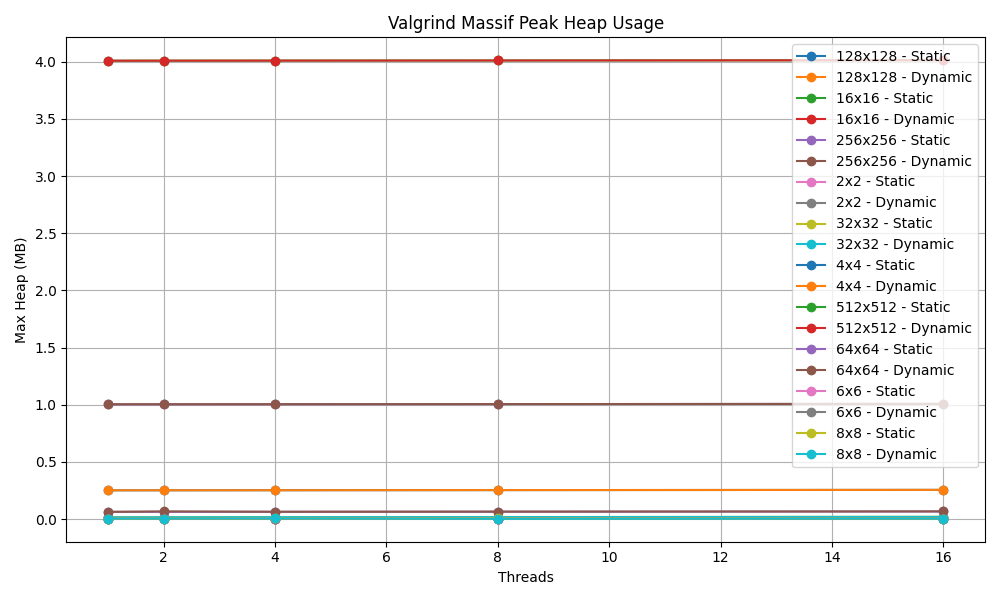
\includegraphics[width=.9\textwidth]{./figure/valgrind_memory_plot.png}
			\caption{各实验的内存对比图}
		\end{minipage}
		\begin{minipage}{.45\textwidth}
			\centering
			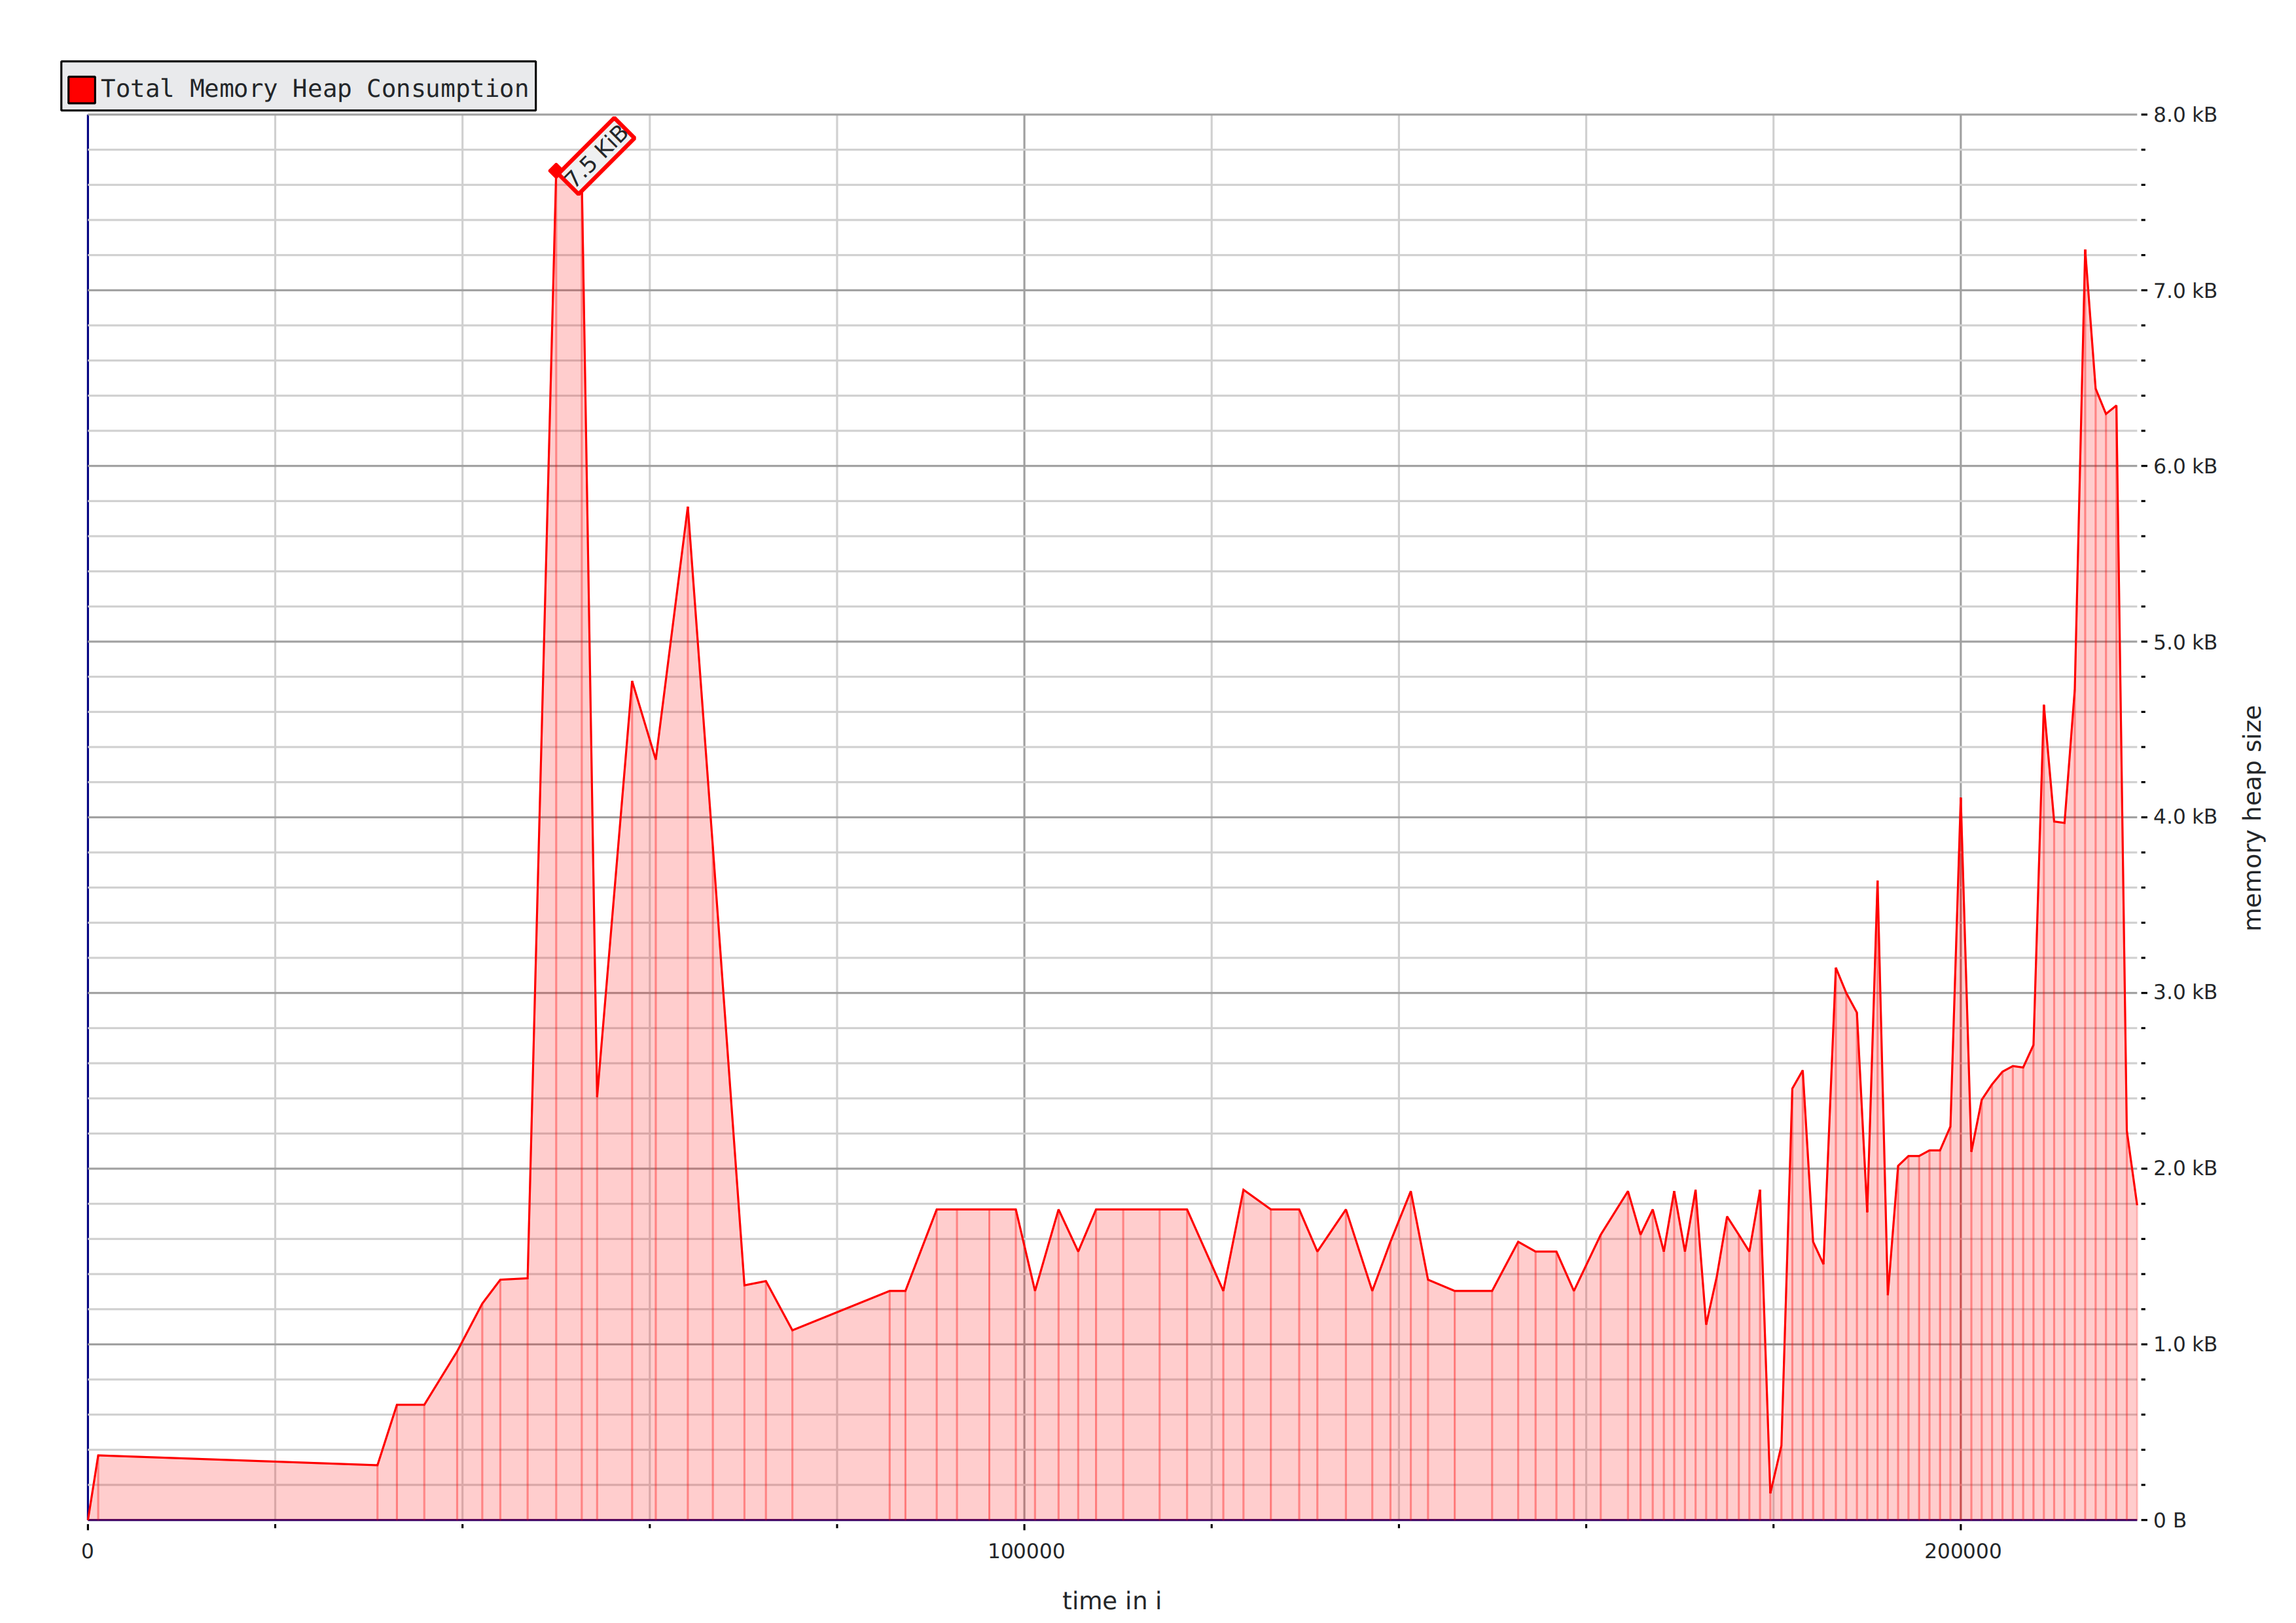
\includegraphics[width=.8\textwidth]{./figure/valgrind_visualize_2_1.png}
			\caption{$2\times2$矩阵1线程内存可视化}
		\end{minipage}
		
		\begin{minipage}{.45\textwidth}
			\centering
			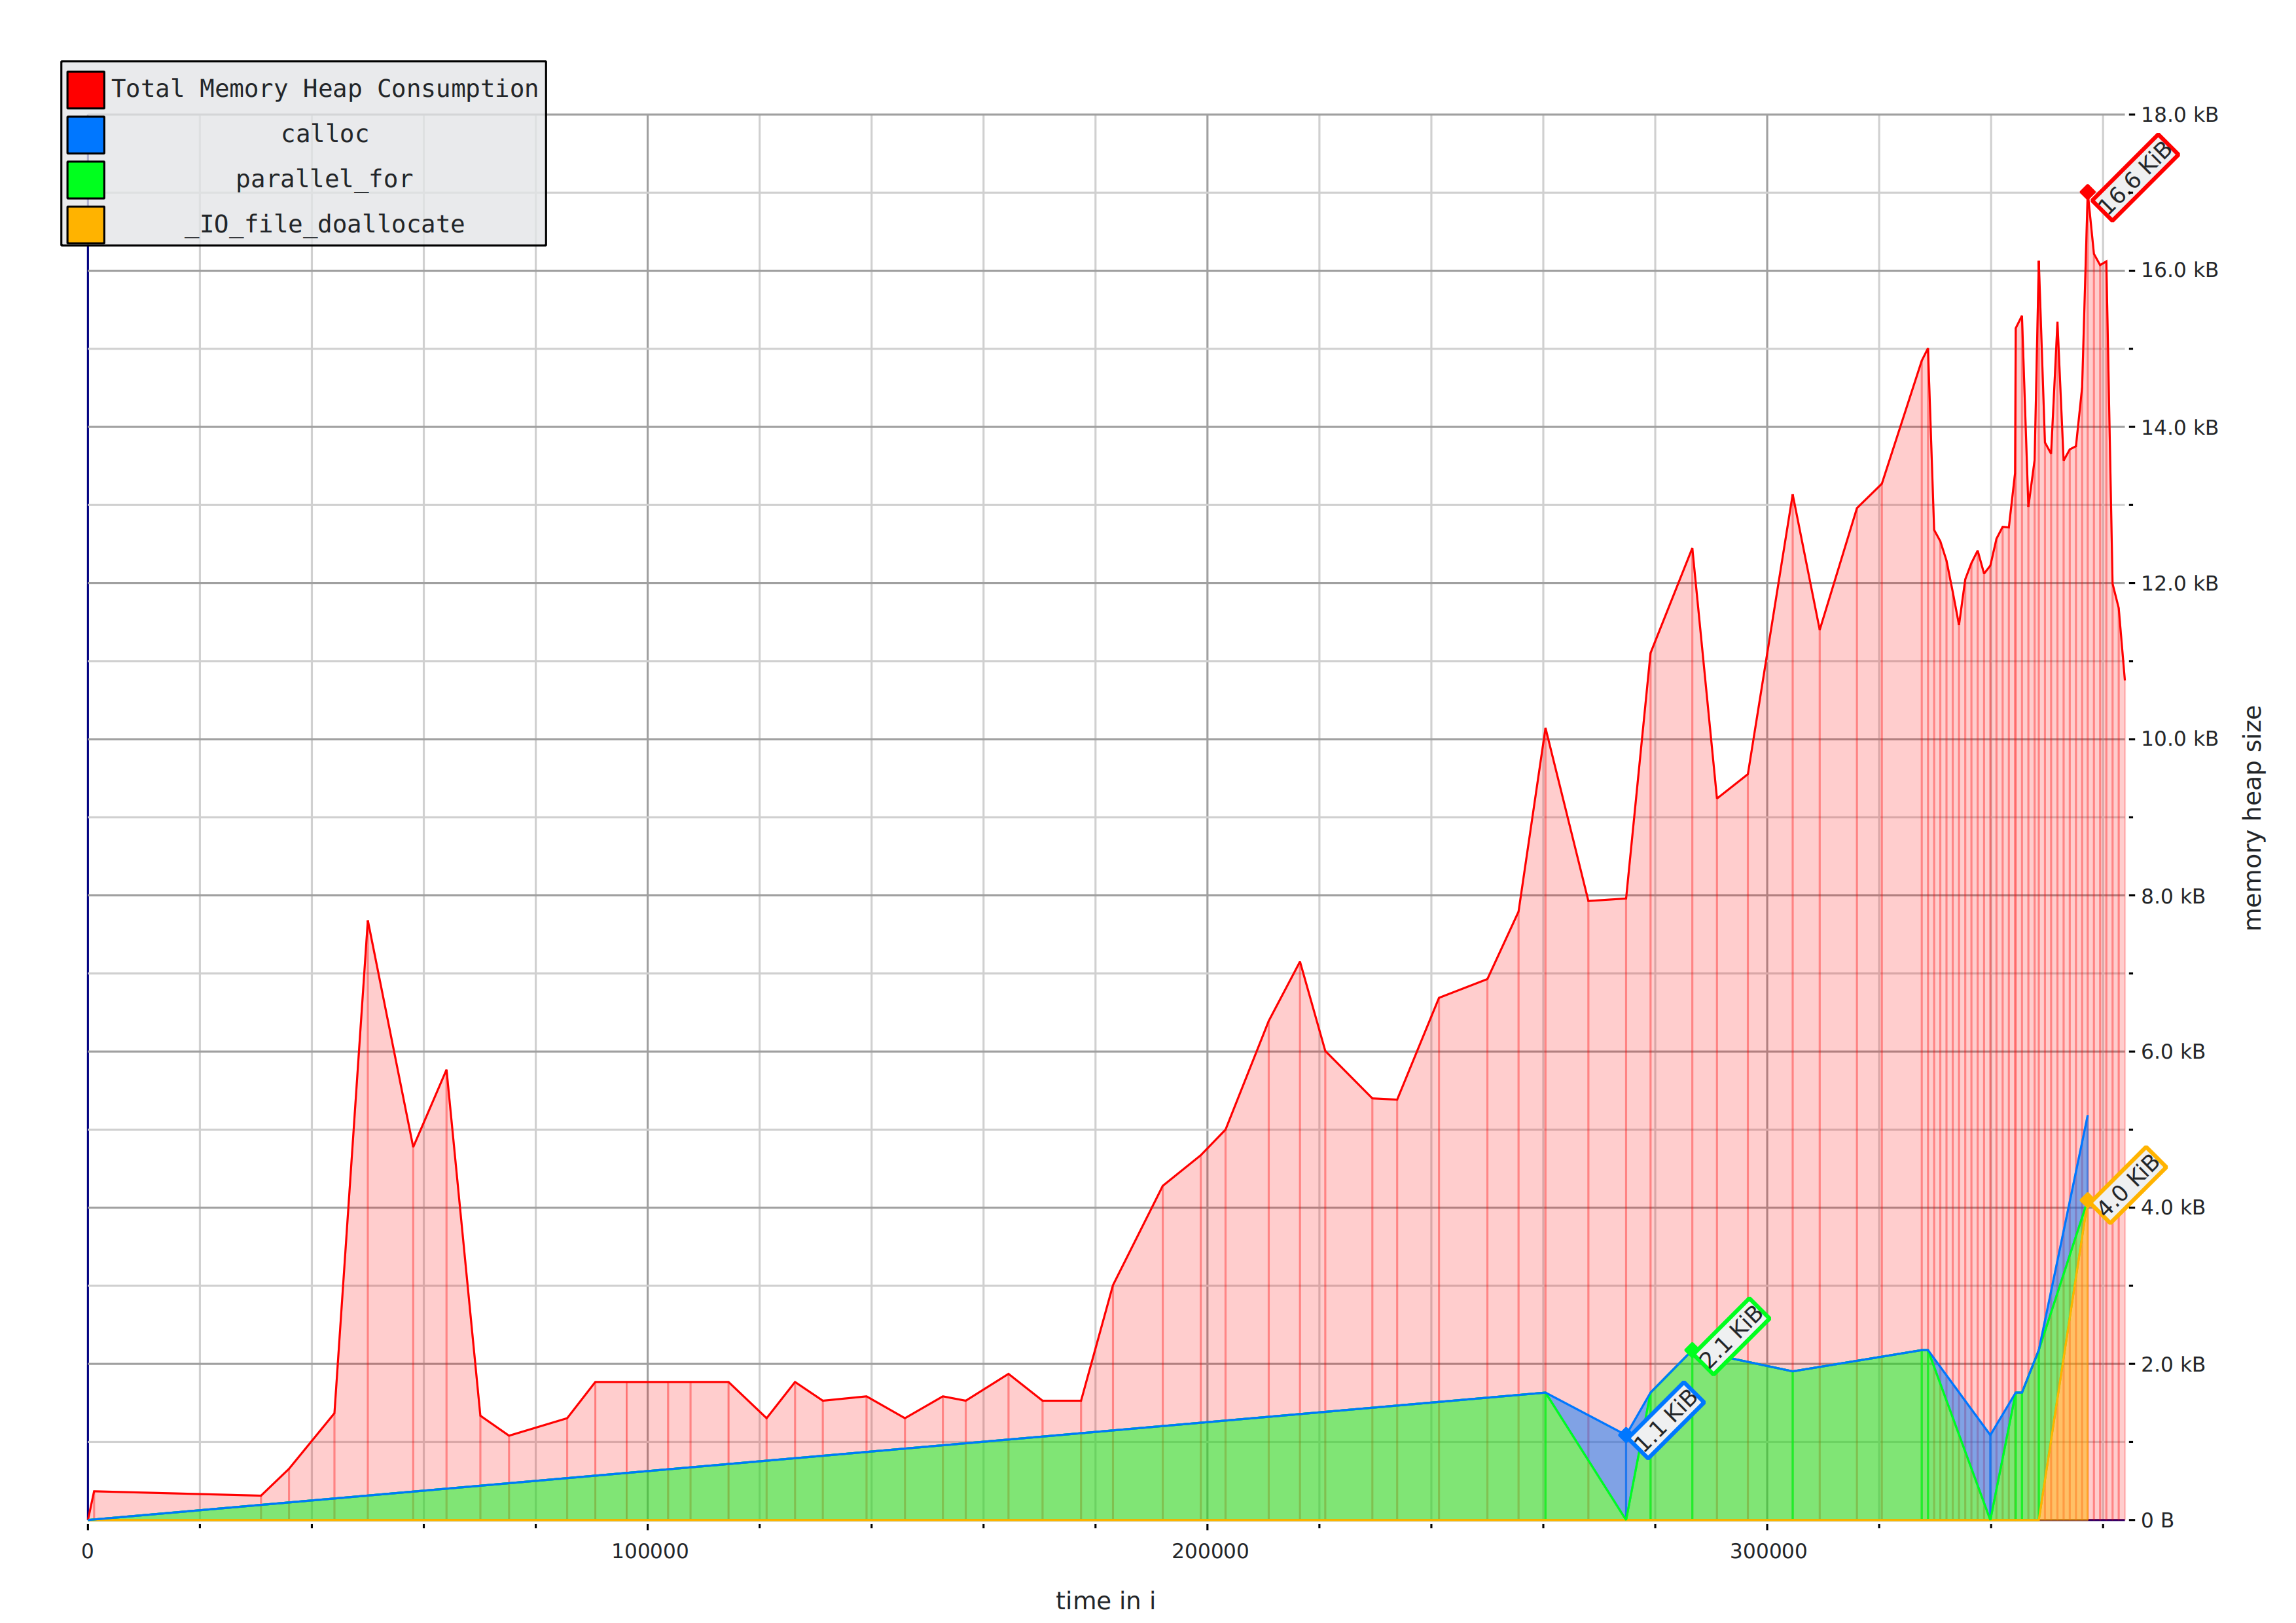
\includegraphics[width=.8\textwidth]{./figure/valgrind_visualize_2_8.png}
			\caption{$2\times2$矩阵8线程内存可视化}
		\end{minipage}
		\begin{minipage}{.45\textwidth}
			\centering
			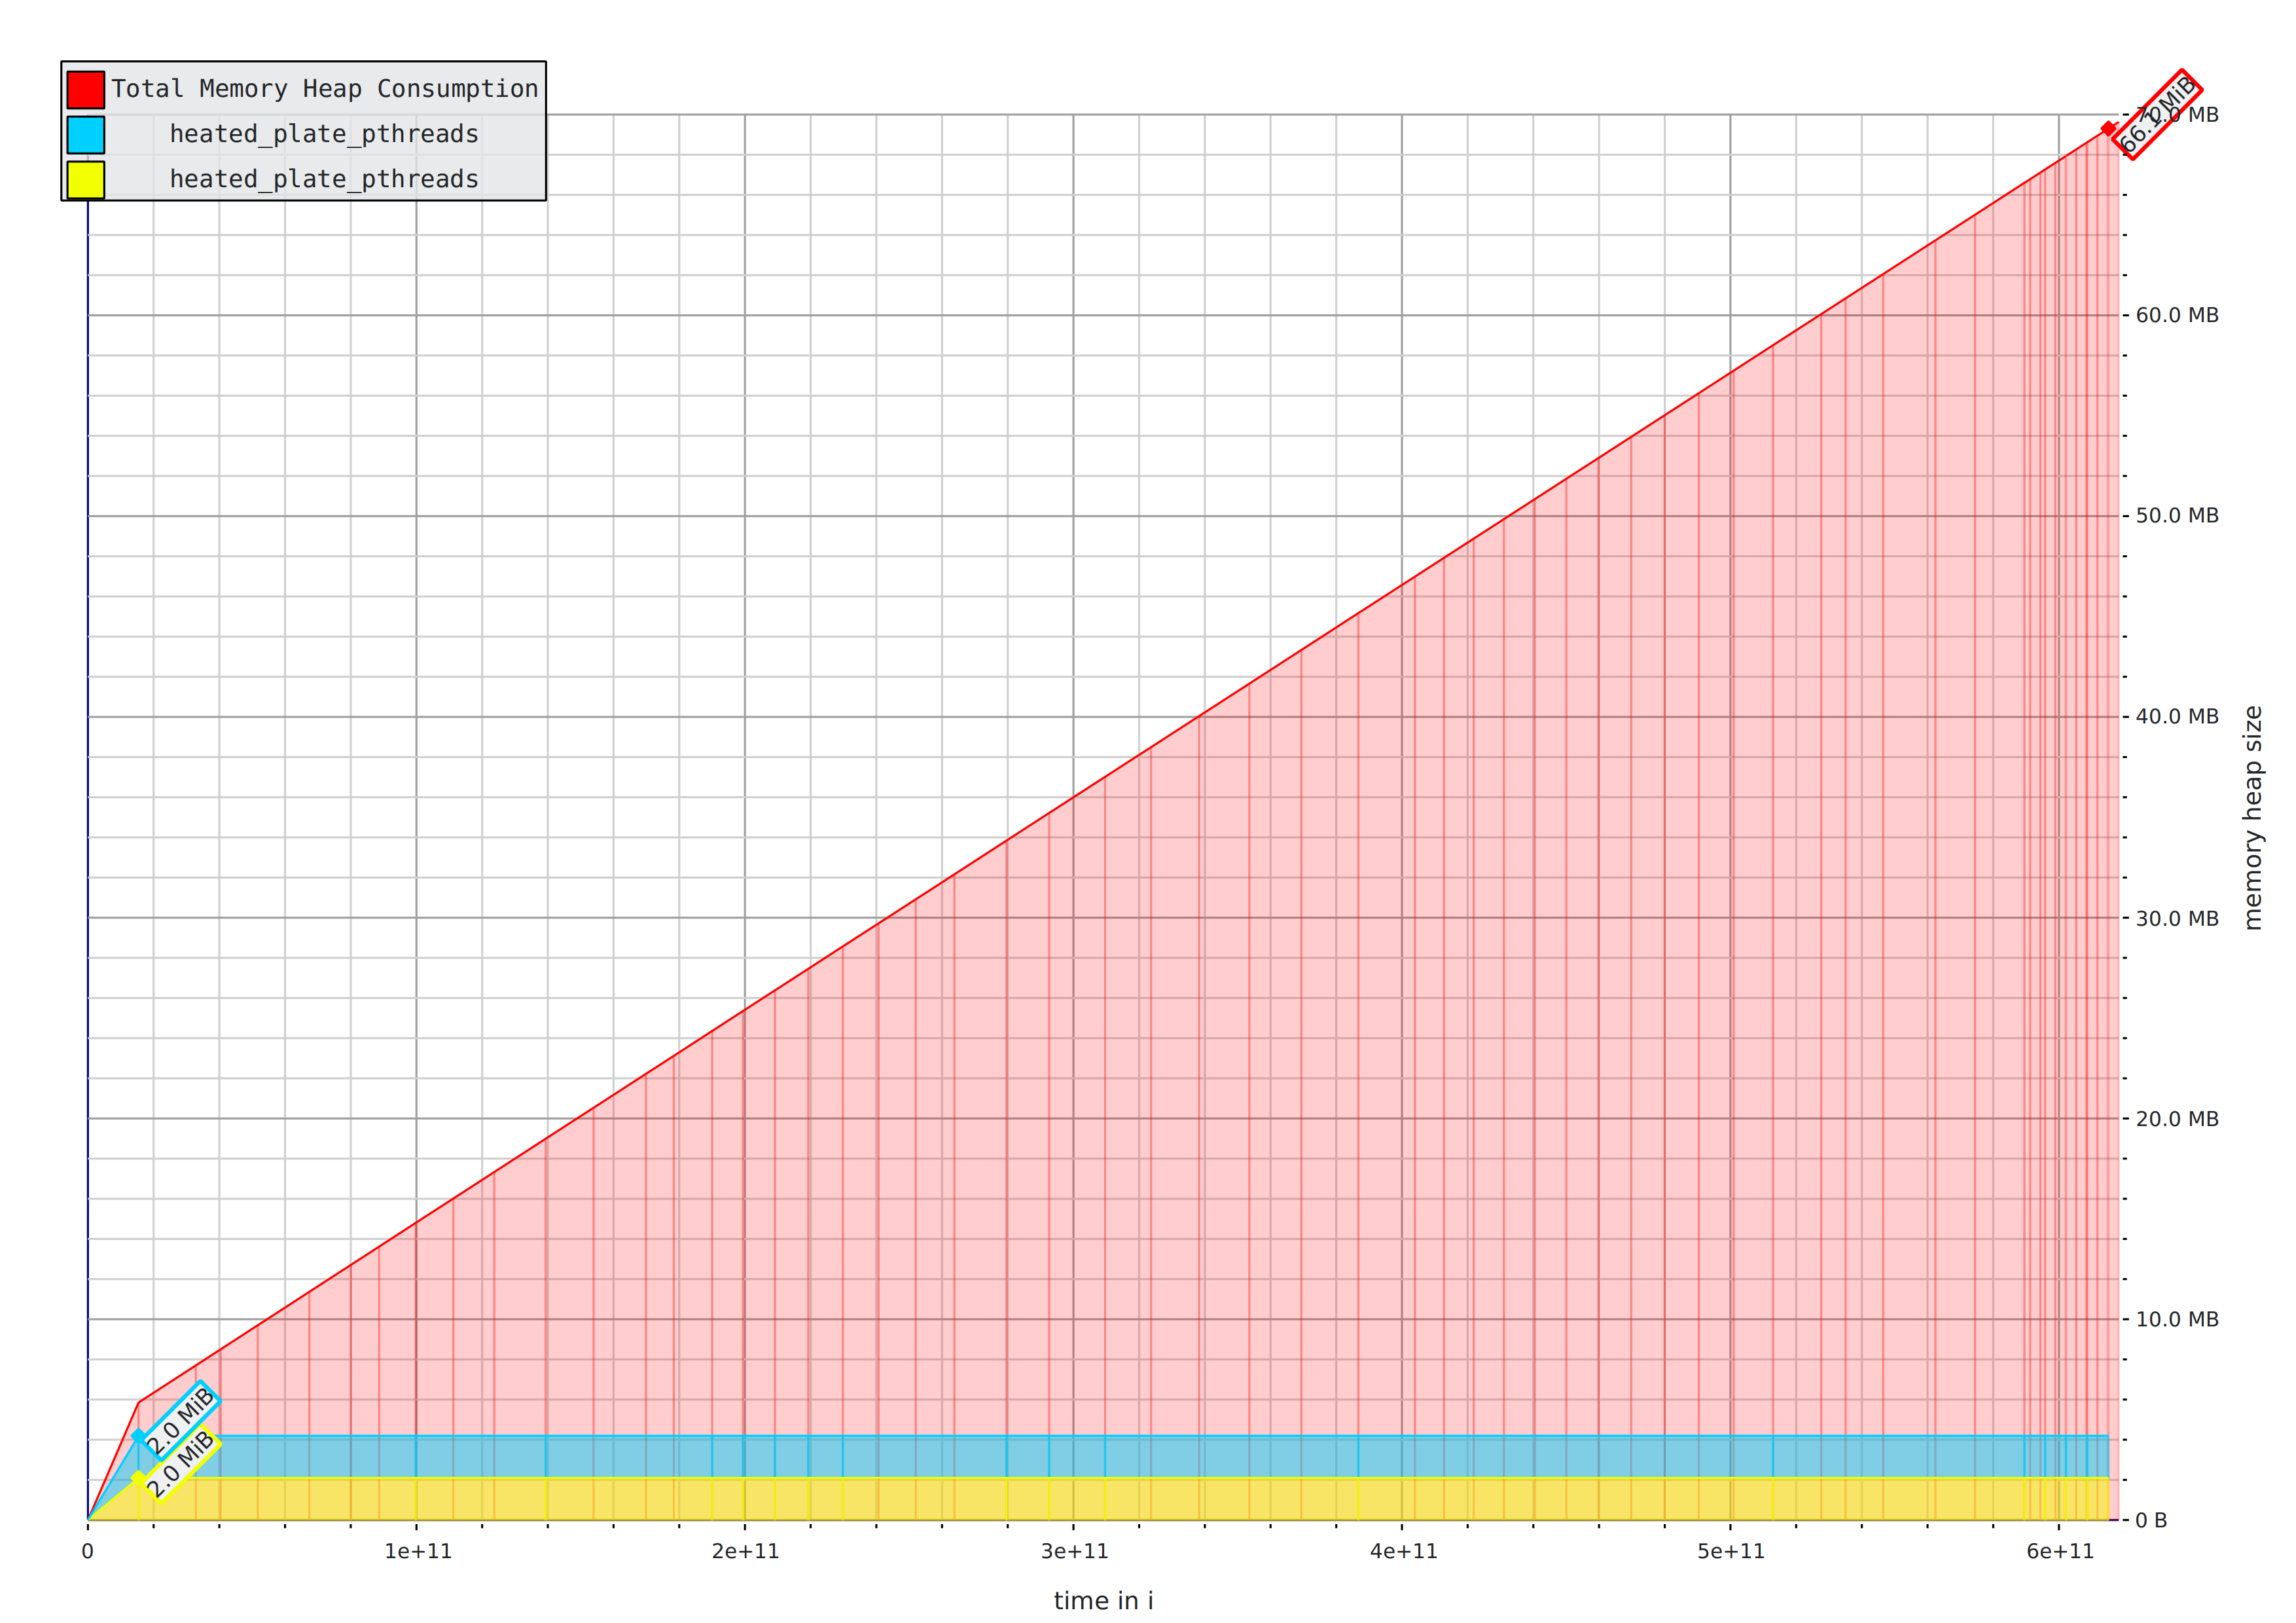
\includegraphics[width=.8\textwidth]{./figure/valgrind_visualize_512_8.png}
			\caption{$512\times512$矩阵8线程内存可视化}
		\end{minipage}
	\end{figure}
	
	此外,内存使用曲线分析显示,程序在运行过程中内存分配较为平稳,峰值出现在特定快照点后保持稳定,无明显的持续增长趋势,证明了内存分配与释放机制工作正常,没有发生明显的内存泄漏。例如,单线程运行时内存峰值约为213.7KB,曲线较平缓,峰值出现在第9号快照后趋于平稳;而多线程处理$512\times512$矩阵时,内存曲线虽出现多次陡升,反映了多阶段大规模内存分配,可能对应于分块计算及线程间缓存数据的分配,但整体趋势依然稳定,未见异常内存泄漏迹象。
	
	综合以上分析,程序内存使用特征合理且表现出良好的扩展性:对于小规模任务,程序保持低内存占用与高效运行;对于大规模、高并发任务,内存峰值虽显著增加,但管理合理,能够有效支持高负载计算环境。该Pthreads并行构造方案在内存资源的管理和利用方面展现出优异的性能,保证了实验任务在不同计算规模和线程数下均能高效稳定运行。
	
	\section{总结与思考}
	
	本实验的目标是通过基于Pthreads的并行程序设计,掌握如何有效地实现并行化计算。通过设计并实现一个通用的\verb|parallel_for|函数,我们成功地将传统的串行矩阵乘法和热传导模拟问题进行了并行化处理,并且对比了不同线程数与调度策略下的性能表现。
	
	从实验结果可以看出,随着线程数的增加,特别是在较大规模任务下,使用Pthreads的并行计算能够显著减少执行时间。在静态调度策略下,线程数的增加带来了较为明显的性能提升,尤其是在大规模任务中,计算时间大幅度下降。然而,在任务规模较小的情况下,线程数的增加并不总是线性地提升性能,这表明系统的资源调度开销和线程管理可能会成为瓶颈,影响并行计算的效率。
	
	相比静态调度,动态调度在处理任务时表现出更高的灵活性和更好的负载均衡,尤其适合任务执行时间不均衡的场景。动态调度策略能够在运行时根据任务需求调整线程的工作负载,避免了某些线程空闲或过度忙碌的情况,从而提升了整体的执行效率。
	
	通过本实验,我们不仅掌握了如何基于Pthreads进行多线程编程,还理解了不同调度策略对并行计算性能的影响。在实际的应用中,选择合适的线程数和调度策略是优化并行计算性能的关键。静态调度适用于任务规模较大的情况,而动态调度则能在任务负载不均的情况下提供更好的性能表现。
	
	最后,虽然我们在本实验中取得了较为理想的性能提升,但仍有一些需要进一步优化的地方。例如,线程数和任务划分的最优策略需要根据具体问题的特点进行调节,并且在高并发场景下,如何避免线程同步开销过大的问题仍是一个值得深入探讨的方向。
	
	\let\cleardoublepage\clearpage
	
	\begin{thebibliography}{99}  
		\bibitem{ref1} 彼得·S·帕切科,\ 马修·马伦塞克.\ 并行程序设计导论[M].\ 黄智濒,\ 肖晨\ 译.\ 原书第2版.\ 北京:机械工业出版社,\ 2024.
		\bibitem{ref2} 黄聃.\ 课件5[EB/OL].\ [2025-3-10].\ https://easyhpc.net/course/221/lesson/1416/material/3173.
		\bibitem{ref3} 黄聃.\ 课件6[EB/OL].\ [2025-3-10].\ https://easyhpc.net/course/221/lesson/1450/material/3182.
	\end{thebibliography}
	
\end{document}
